%!TEX program = xelatex
%%%%%%%%%%%%%%%%%%%%%%%这是导言部分的开始%%%%%%%%

%========= 导言部分声明文档的类型=================
\documentclass{article}

	%=========导言部分可可以加载宏包=================
	\usepackage{amsmath}                % 数学公式排版宏包
	\usepackage{amssymb}                % 数学符号命令宏包
	\usepackage{amsthm}                 % 数学定理宏包
	\usepackage[UTF8]{ctex}             % 中文输入宏包
	\usepackage[a4paper]{geometry}      % 页面设置宏包
	\usepackage{setspace}               % 行间距宏包
	\usepackage{graphicx}               % 图片宏包
	\usepackage{listings}               % 代码宏包
	\usepackage{color}					% 颜色宏包
	\usepackage{xcolor}                 % 颜色处理宏包
	\usepackage{float}                  % 浮动对象式样宏包
	\usepackage{fontspec}
	\usepackage{enumerate}				% 列举编号包
	
	%=========页面设置==============================
	\geometry{left=1cm,right=1cm,top=1cm,bottom=2cm}
	\onehalfspacing
	\setlength\parindent{0em}

	%=========代码格式设置============================
	\definecolor{dkgreen}{rgb}{0,0.6,0}
	\definecolor{gray}{rgb}{0.5,0.5,0.5}
	\definecolor{mauve}{rgb}{0.58,0,0.82}
	% \setmonofont{Consolas}
	\lstset{
		numbers = left, 	
		numberstyle = \color{gray}, 
		keywordstyle = \color{blue},
		commentstyle = \color{dkgreen}, 
		stringstyle = \color{mauve},
		basicstyle = \ttfamily,
		breaklines = true,
		frame = shadowbox, % 阴影效果
		rulesepcolor = \color{ red!20!green!20!blue!20} ,
		escapeinside = ``, % 英文分号中可写入中文
		xleftmargin = 2em,xrightmargin=2em, aboveskip=1em,
		framexleftmargin = 2em
	} 

%=========导言部分可以定义标题信息===============
\title{组会报告}
\author{徐益}
\date{\today}
%%%%%%%%%%%%%%%%%%%%%%%这是导言部分的结束%%%%%%%%%

%%%%%%%%%%%%%%%%%%%%%%%这是正文部分的开始%%%%%%%%%
\begin{document}

%=========生成标题================================
\maketitle

%=========开始正文的输入==========================

%===========第一节=================
\section{工作内容}
1. 对107/108两台服务器上的icc进行修复;

2. 按要求对test\_5g\_simd\_ldpc系统代码进行改写;

3. 解决fixed译码中的误码性能“平台”问题;

4. 完成部分仿真报告。

%===========第一节=================
\section{编码部分的SIMD改写}
\lstset{language=C++}
\begin{lstlisting}
void circshift_xor_avx2(int8_t *dst, int8_t *src, int32_t num, int32_t len)
{
	int32_t i;
	int32_t loop1_32, loop1_1, loop2_32, loop2_1;
	int8_t *p_src, *p_dst;
	__m256i vsrc, vdst;

	loop1_32 = (len - num) / REG_SIZE;
	loop1_1 = (len - num) % REG_SIZE;
	loop2_32 = num / REG_SIZE;
	loop2_1 = num % REG_SIZE;

	p_dst = dst;
	p_src = src + num;
	for (i = 0; i < loop1_32; i++)
	{
		vdst = VECTOR_LOAD((__m256i *)p_dst);
		vsrc = VECTOR_LOAD((__m256i *)p_src);
		vdst = VECTOR_XOR(vdst, vsrc);
		VECTOR_STORE((__m256i *)p_dst, vdst);
		p_dst += REG_SIZE;
		p_src += REG_SIZE;
	}
	for (i = 0; i < loop1_1; i++)
	{
		*p_dst ^= *p_src;
		p_dst++;
		p_src++;
	}
	p_src = src;
	for (i = 0; i < loop2_32; i++)
	{
		vdst = VECTOR_LOAD((__m256i *)p_dst);
		vsrc = VECTOR_LOAD((__m256i *)p_src);
		vdst = VECTOR_XOR(vdst, vsrc);
		VECTOR_STORE((__m256i *)p_dst, vdst);
		p_dst += REG_SIZE;
		p_src += REG_SIZE;
	}
	for (i = 0; i < loop2_1; i++)
	{
		*p_dst ^= *p_src;
		p_dst++;
		p_src++;
	}
}
\end{lstlisting}

%===========第二节=================
\section{“平台”问题的解决}
\subsection{问题}
\begin{figure}[H]
	\centering
	\includegraphics[width = .8\textwidth]{err.eps}
	\caption{出现平台问题的误码性能图}
\end{figure}
\subsection{出现问题的原因和解决方法}
问题原因:部分点的对数似然比锁定为0。\\
解决方法:调制限幅参数。\\
\lstset{language=C++}
\begin{lstlisting}
#define FACTOR_BETA 4
\end{lstlisting}
\subsection{修改后结果}
\begin{figure}[H]
	\centering
	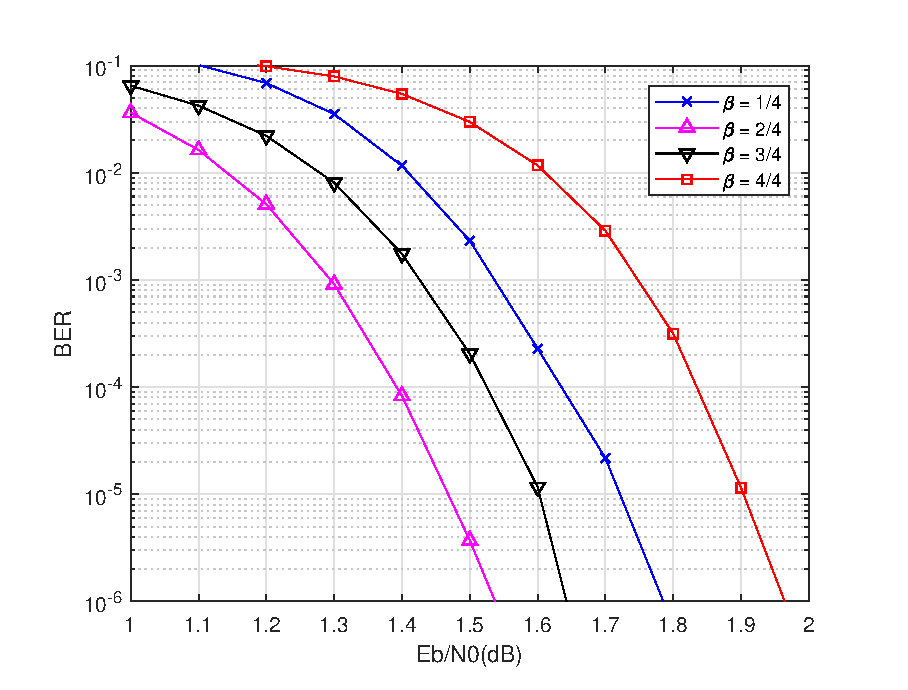
\includegraphics[width = .8\textwidth]{oms.eps}
	\caption{不同参数下的OMS误码性能对比($N=16896, R=0.5$)}
\end{figure}
\begin{figure}[H]
	\centering
	\includegraphics[width = .8\textwidth]{nms.eps}
	\caption{不同参数下的NMS误码性能对比($N=16896, R=0.5$)}
\end{figure}

%===========第三节=================
\section{仿真报告}



%===========第四节=================
% \section{仍存在的问题}


%===========下周计划=================
% \section{下阶段计划}
% 1. 继续完成仿真报告

\end{document}
%%%%%%%%%%%%%%%%%%%%%%%这是正文部分的结束%%%%%%%%%%%%